\pdfminorversion=4
\documentclass[aspectratio=169]{beamer}

\mode<presentation>
{
  \usetheme{default}
  \usecolortheme{default}
  \usefonttheme{default}
  \setbeamertemplate{navigation symbols}{}
  \setbeamertemplate{caption}[numbered]
  \setbeamertemplate{footline}[frame number]  % or "page number"
  \setbeamercolor{frametitle}{fg=white}
  \setbeamercolor{footline}{fg=black}
} 

\usepackage[english]{babel}
\usepackage[utf8x]{inputenc}
\usepackage{tikz}
\usepackage{courier}
\usepackage{array}
\usepackage{bold-extra}
\usepackage{minted}
\usepackage[thicklines]{cancel}
\usepackage{fancyvrb}

\xdefinecolor{dianablue}{rgb}{0.18,0.24,0.31}
\xdefinecolor{darkblue}{rgb}{0.1,0.1,0.7}
\xdefinecolor{darkgreen}{rgb}{0,0.5,0}
\xdefinecolor{darkgrey}{rgb}{0.35,0.35,0.35}
\xdefinecolor{darkorange}{rgb}{0.8,0.5,0}
\xdefinecolor{darkred}{rgb}{0.7,0,0}
\definecolor{darkgreen}{rgb}{0,0.6,0}
\definecolor{mauve}{rgb}{0.58,0,0.82}

\title[2018-11-07-hsf-hep-in-numpy]{HEP analysis in the Numpy ecosystem}
\author{Jim Pivarski}
\institute{Princeton University -- DIANA-HEP}
\date{November 7, 2018}

\usetikzlibrary{shapes.callouts}

\begin{document}

\logo{\pgfputat{\pgfxy(0.11, 7.4)}{\pgfbox[right,base]{\tikz{\filldraw[fill=dianablue, draw=none] (0 cm, 0 cm) rectangle (50 cm, 1 cm);}\mbox{\hspace{-8 cm}
\includegraphics[height=1 cm]{princeton-logo-long.png}
\includegraphics[height=1 cm]{diana-hep-logo-long.png}}}}}

\begin{frame}
  \titlepage
\end{frame}

\logo{\pgfputat{\pgfxy(0.11, 7.4)}{\pgfbox[right,base]{\tikz{\filldraw[fill=dianablue, draw=none] (0 cm, 0 cm) rectangle (50 cm, 1 cm);}\mbox{\hspace{-8 cm}
\includegraphics[height=1 cm]{princeton-logo.png}
\includegraphics[height=1 cm]{diana-hep-logo.png}}}}}

% Uncomment these lines for an automatically generated outline.
%\begin{frame}{Outline}
%  \tableofcontents
%\end{frame}

% START START START START START START START START START START START START START

\begin{frame}{In case we need a ``Motivations'' section}
\vspace{0.25 cm}
\begin{center}
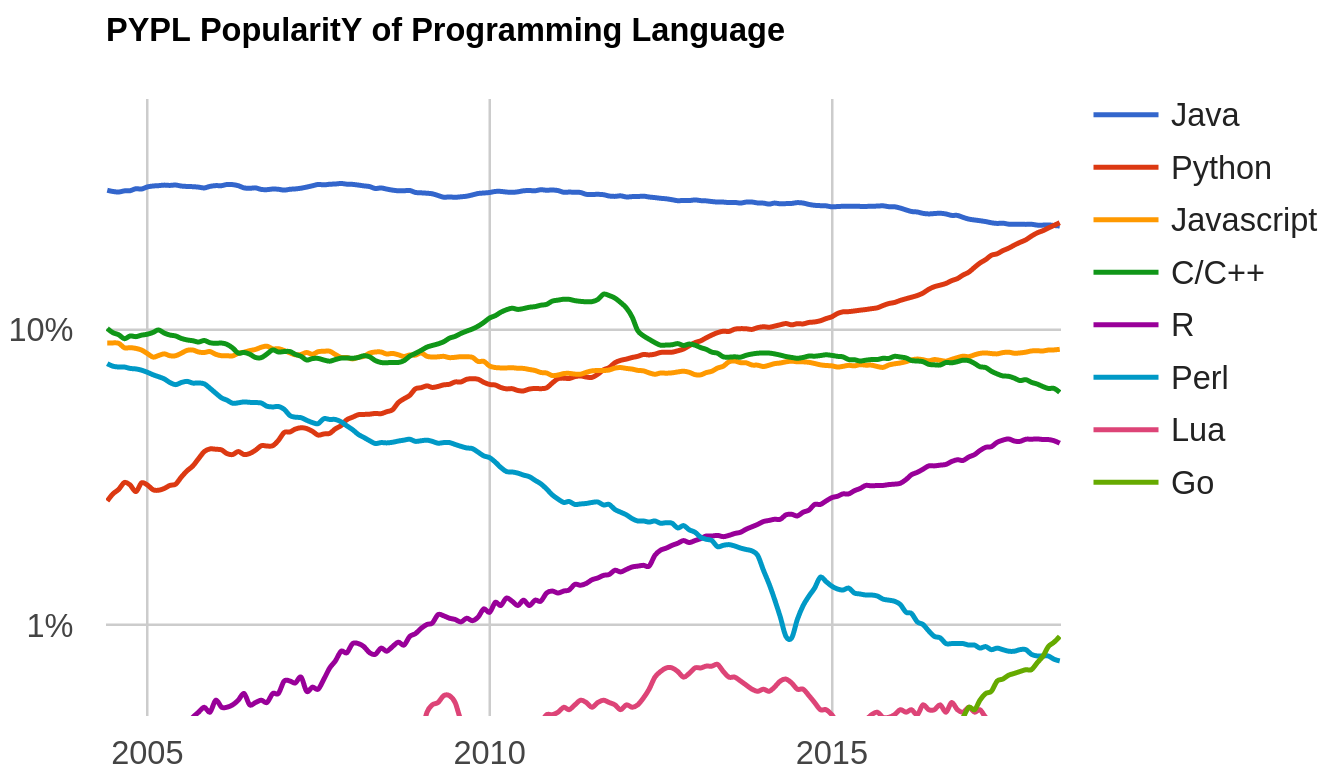
\includegraphics[width=0.8\linewidth]{pypl-popularity.png}
\end{center}
\textcolor{blue}{\scriptsize\url{http://pypl.github.io/PYPL.html}}
\end{frame}

\begin{frame}{In case we need a ``Motivations'' section}
\vspace{0.5 cm}
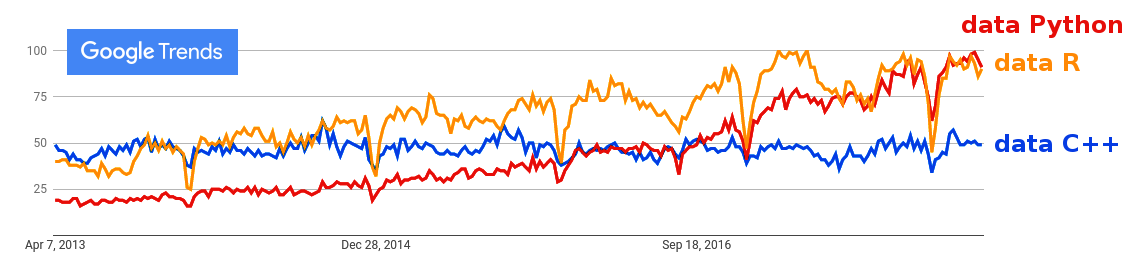
\includegraphics[width=\linewidth]{python-r-cpp-googletrends-data.png}

\vspace{1 cm}
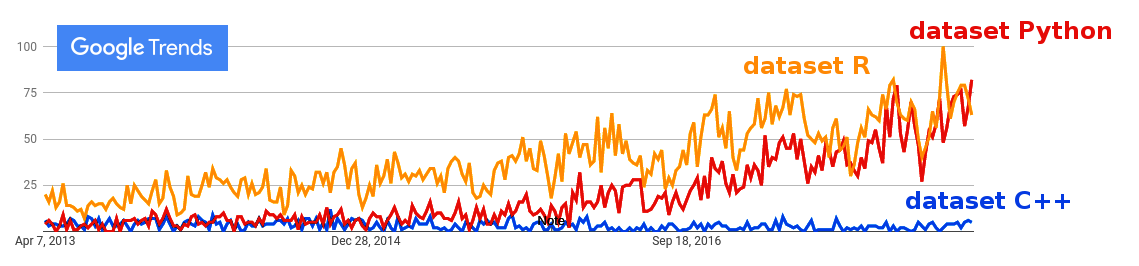
\includegraphics[width=\linewidth]{python-r-cpp-googletrends-dataset.png}
\end{frame}

\begin{frame}{In case we need a ``Motivations'' section}
\vspace{0.5 cm}
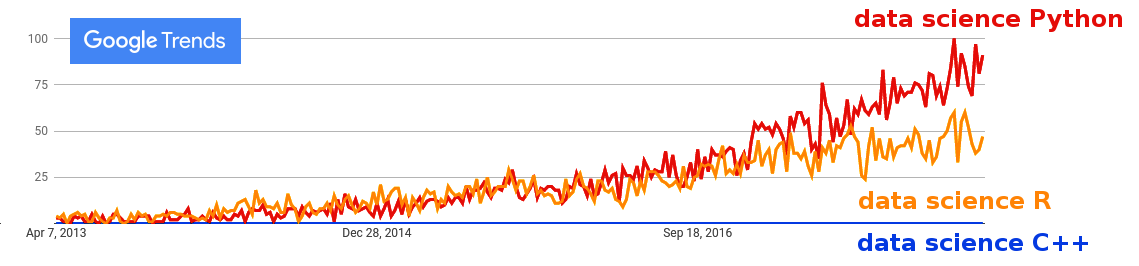
\includegraphics[width=\linewidth]{python-r-cpp-googletrends-datascience.png}

\vspace{1 cm}
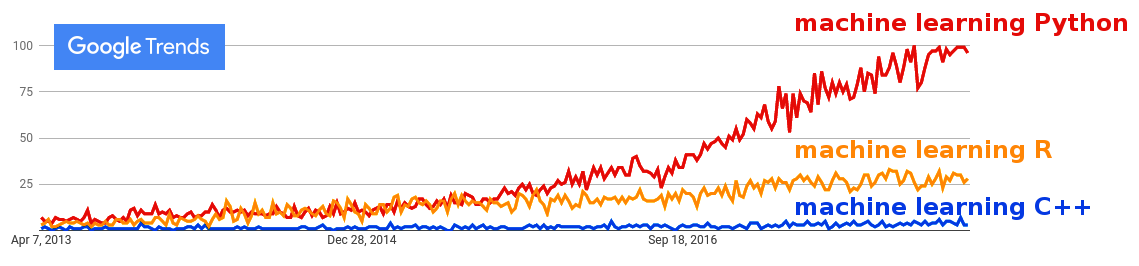
\includegraphics[width=\linewidth]{python-r-cpp-googletrends-machinelearning.png}
\end{frame}

\begin{frame}{In case we need a ``Motivations'' section}
\vspace{0.5 cm}
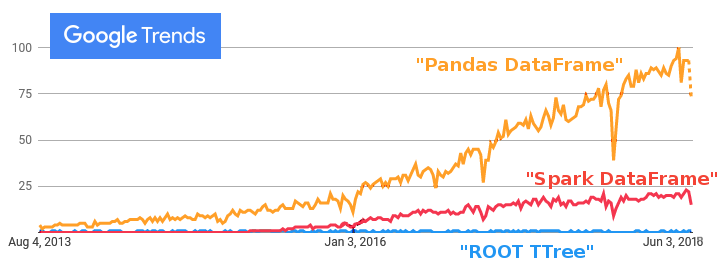
\includegraphics[width=\linewidth]{root-spark-pandas-google-trends.png}
\end{frame}

\begin{frame}{Stealing from Jake VanderPlas's {\it Unexpected Effectiveness} talk}
\vspace{0.25 cm}
\begin{columns}[b]
\column{0.75\linewidth}
\only<1>{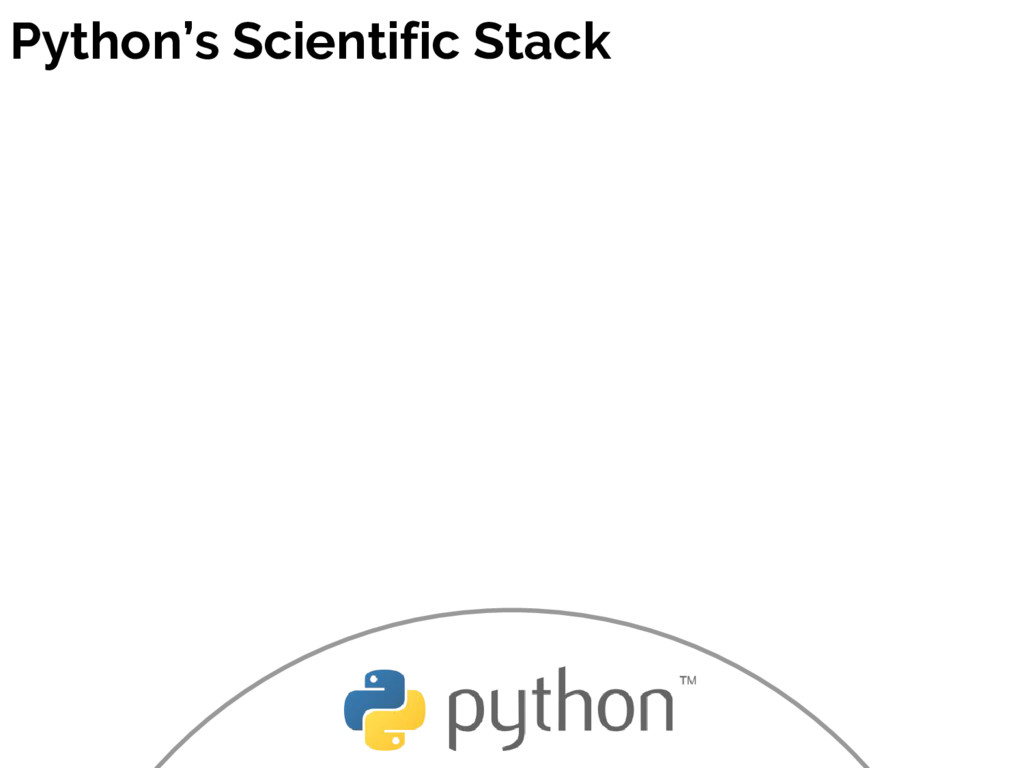
\includegraphics[height=7.8 cm]{shells-1.png}}
\only<2>{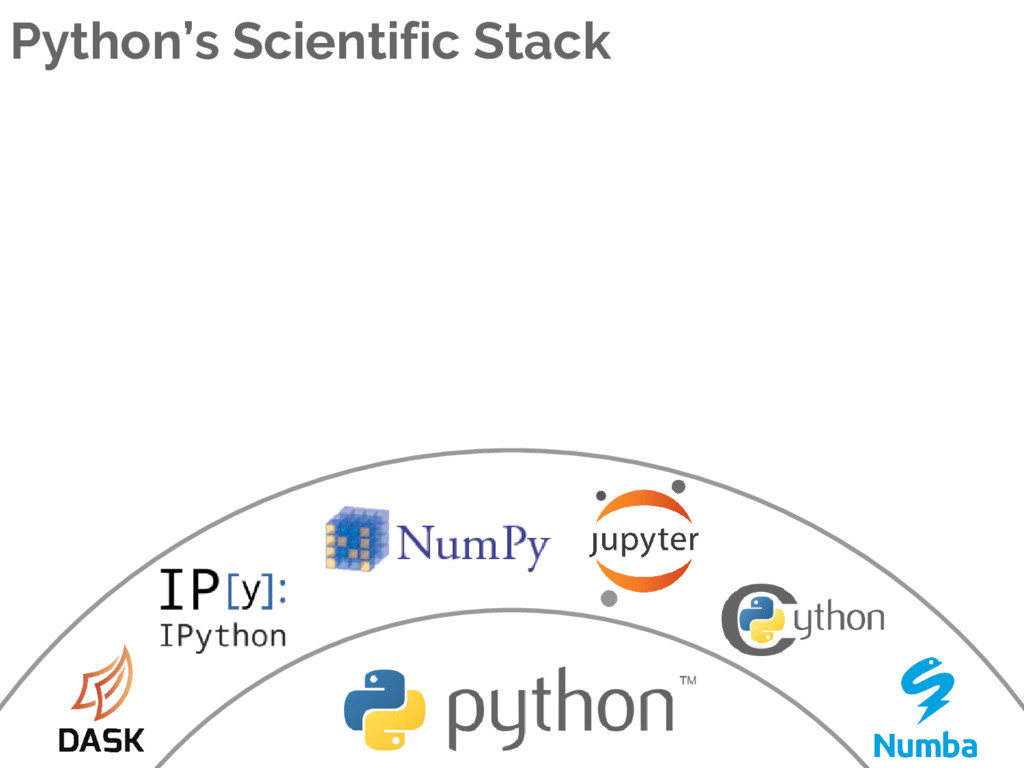
\includegraphics[height=7.8 cm]{shells-2.png}}
\only<3>{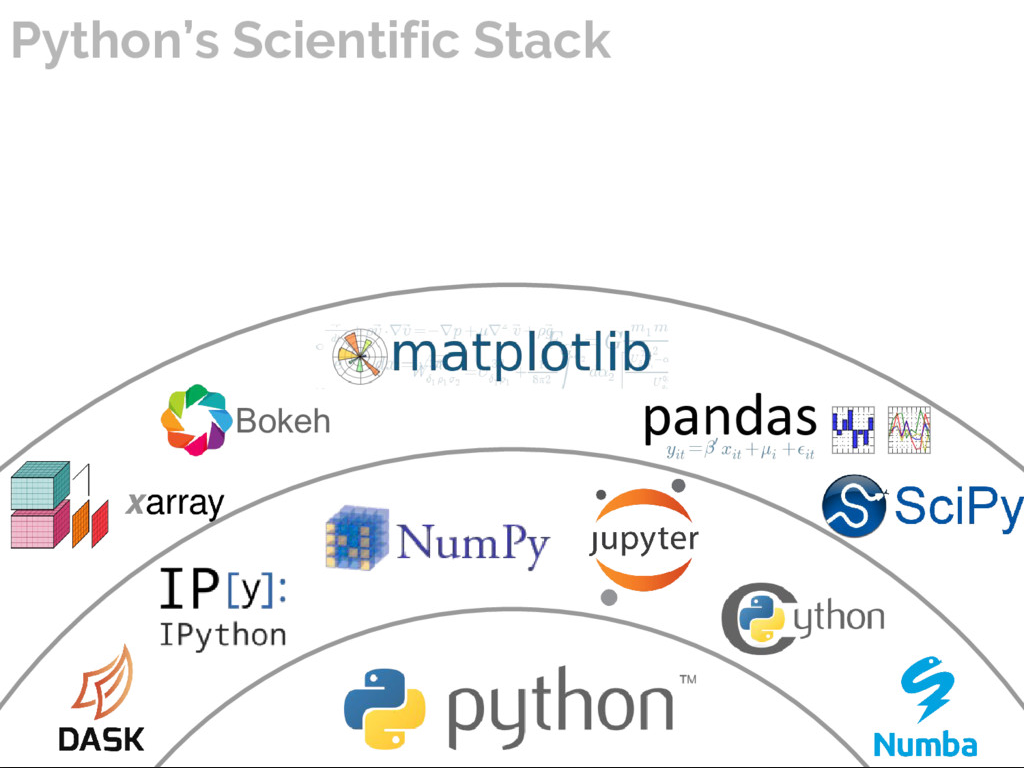
\includegraphics[height=7.8 cm]{shells-3.png}}
\only<4>{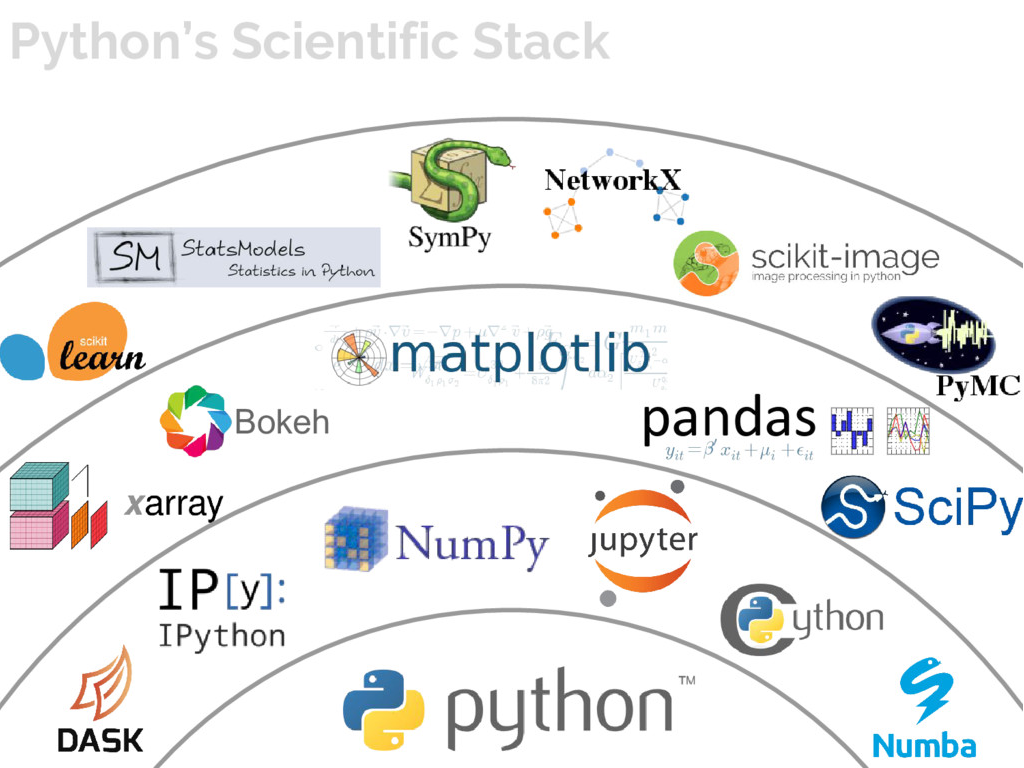
\includegraphics[height=7.8 cm]{shells-4.png}}
\only<5>{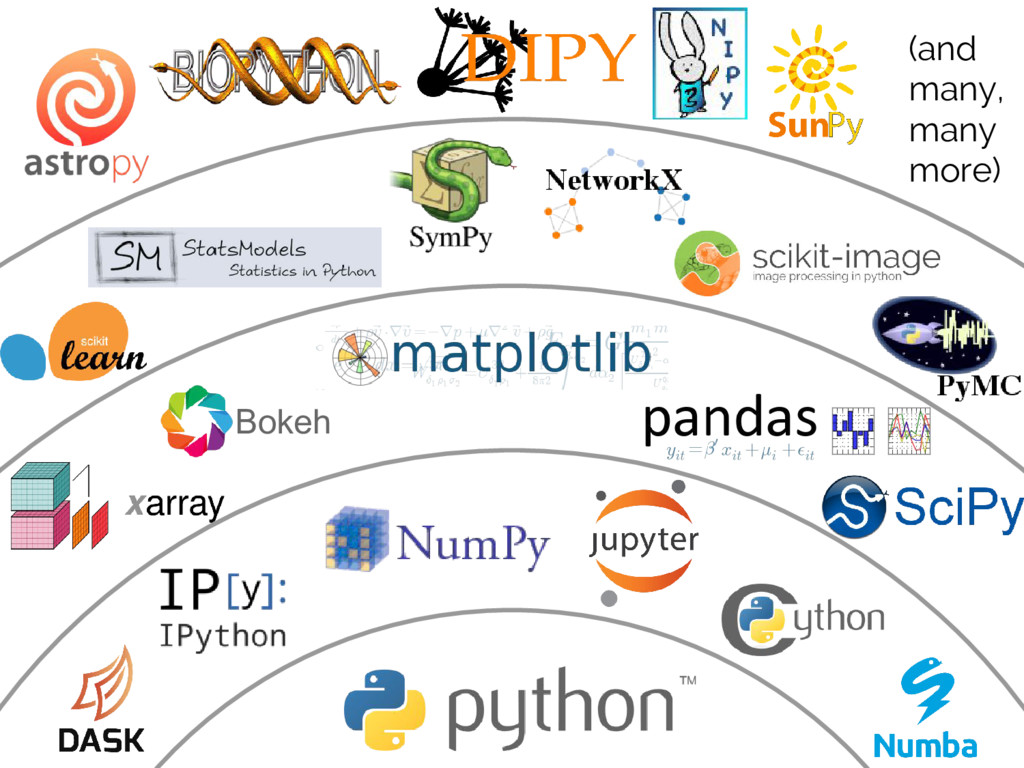
\includegraphics[height=7.8 cm]{shells-5.png}\vspace{0.5 cm}}

\column{0.25\linewidth}

\includegraphics[width=\linewidth]{unreasonable-effectiveness.png}
\vspace{5.3 cm}
\end{columns}
\end{frame}

\begin{frame}{The other sciences are doing it, so why can't I?}
\vspace{0.3 cm}
\begin{columns}[b]
\column{0.59\linewidth}
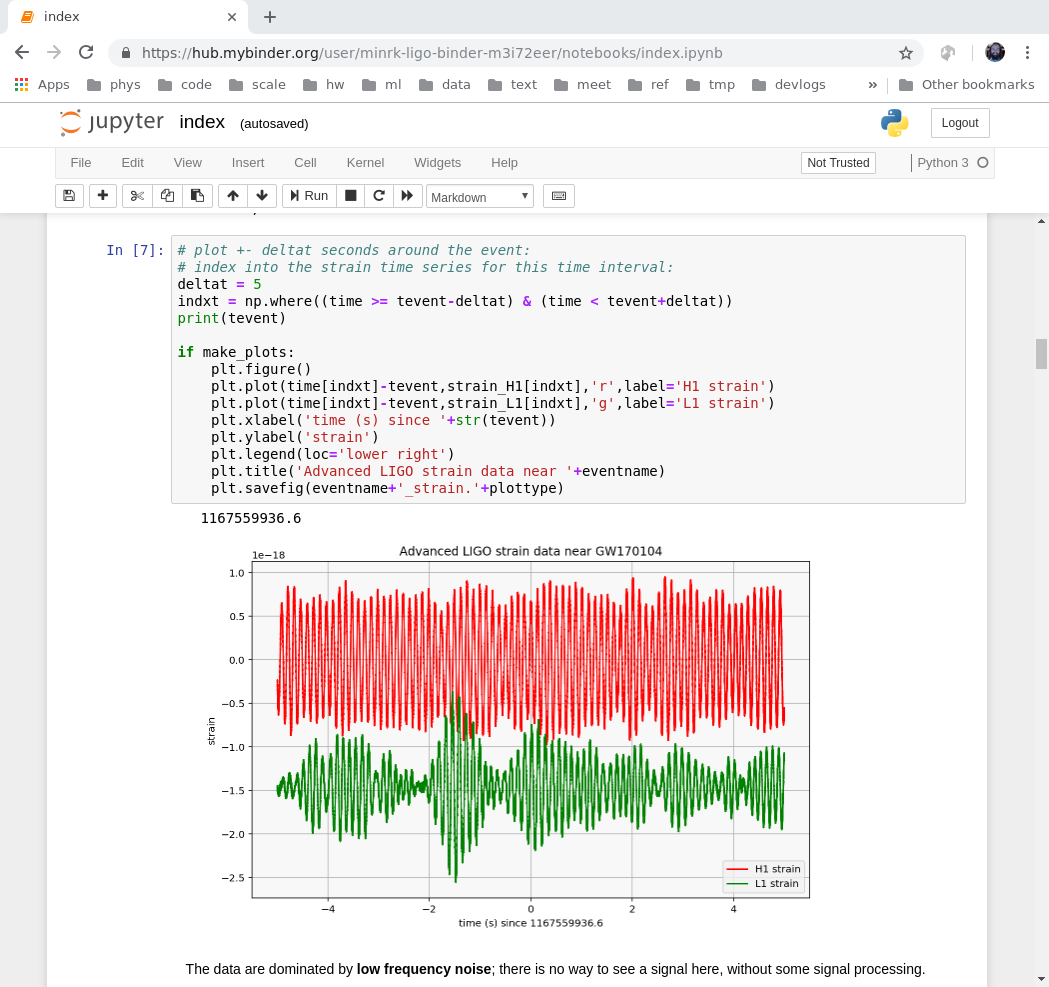
\includegraphics[width=\linewidth]{lsst-notebook.png}

\column{0.41\linewidth}
\begin{itemize}\setlength{\itemsep}{0.5 cm}
\item LIGO full analysis in \\ Numpy $+$ Jupyter $+$ Binder \\ $\to$ you can run all the signal processing yourself without downloading anything.
\item LSST is adopting Python $+$ Jupyter as the general astronomer's interface.
\item XENON-nT is doing their full stack in Python $+$ Numpy.
\item (easy to find examples\ldots)
\end{itemize}

\vspace{0.75 cm}
\end{columns}
\end{frame}

\begin{frame}{Why not indeed?}
\vspace{0.5 cm}
Numpy allowed Python to fill a niche occupied by MATLAB and R: transforming, filtering, signal processing, and machine learning on GB's of rectangular array data.

\vspace{0.75 cm}
\begin{columns}[t]
\column{0.1\linewidth}

\column{0.3\linewidth}
\textcolor{darkgreen}{\bf Python for loops are expressive but not fast.}

\vspace{0.25 cm}
Good for small, complex processing that needs a fully nested object model.

\column{0.3\linewidth}
\textcolor{darkorange}{\bf Numpy arrays are \\ fast but not expressive.}

\vspace{0.25 cm}
Good for biggish, more regular processing (including ML).

\column{0.1\linewidth}
\end{columns}

\vspace{0.75 cm}
Most astronomy, data science, etc.\ fits one of these cases.
\end{frame}

\begin{frame}{Three surmountable challenges}
\large
\vspace{0.5 cm}
\begin{center}
\begin{minipage}{0.75\linewidth}
\begin{enumerate}\setlength{\itemsep}{1 cm}
\item HEP software stacks and conventions were developed {\it before} the Numpy ecosystem and have to be retrofitted to communicate easily.

\item HEP analysis relies heavily on nested data: each event may have a different number of particles.

\item HEP analysis must be performed on TB of ntuples or PB of centrally produced data with thousands of users hitting the same system/files.
\end{enumerate}
\end{minipage}\mbox{\hspace{1 cm}}
\end{center}
\end{frame}

\begin{frame}{}
\LARGE
\vspace{1 cm}
\begin{center}
\textcolor{darkblue}{1. HEP software $\leftrightarrow$ Numpy}
\end{center}
\end{frame}

\begin{frame}{An active area for a long time and now accelerating}
\vspace{0.5 cm}
\begin{itemize}\setlength{\itemsep}{0.5 cm}
\item The PyROOT project started in 2003, just before release 2.3 of \raisebox{-0.2\height}{
\includegraphics[height=\baselineskip]{old-python-logo.png}}.

Every C++ class/function is accessible in Python, at a performance price.

\item Many small HEP packages address specific access issues:

\vspace{0.05 cm}
\begin{itemize}\setlength{\itemsep}{0.05 cm}
\item PyMinuit: extracted from my HEP analysis and open sourced in 2005
\item iminuit: modern version, used in astronomy
\item rootpy: more ``Pythonic'' interface overlaid on PyROOT
\item root\_numpy: faster bindings compiled into C++
\item 81 packages matching ``HEP'' in PyPI, 247 in GitHub\ldots
\end{itemize}

\item The ROOT team is actively adding ``Pythonizations'' to PyROOT for a more Pythonic interface and also direct-to-Numpy access.

\vspace{0.1 cm}
\begin{itemize}\setlength{\itemsep}{0.1 cm}
\item {\tt\small ttree.AsMatrix()}: access TTree data in Python as Numpy
\item RDataFrame sources and sinks to include Numpy arrays and Arrow
\end{itemize}
\end{itemize}
\end{frame}





\end{document}
